\documentclass[border=10pt]{standalone}

\usepackage{tikz}
\usetikzlibrary{arrows.meta,arrows,decorations.pathmorphing,backgrounds,positioning,fit,petri,calc,shapes.geometric,scopes,fit,spy,chains}
\usepackage{pgfplots}
\pgfplotsset{,compat=1.11}
\tikzset{/pgf/number format/1000 sep={\,}}

\usepackage{fontawesome5}
\renewcommand{\familydefault}{\sfdefault}
\usepackage{helvet}
\begin{document}

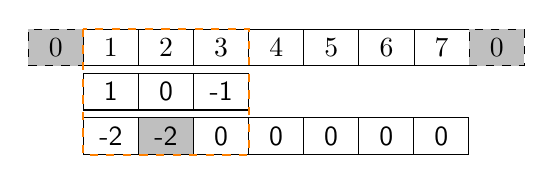
\begin{tikzpicture}[start chain=1 going right,%
        start chain=2 going right,%
        node distance=-0.15mm, %
        minimum width=.7cm,
        auto]

        %\node [dashed, fill=lightgray,draw] (ghost_li0_1) at(0,0) {$0$};
        %% second line
        \node [dashed, fill=lightgray,draw] (ghost_li1_1) at(0,0) {$0$};
        \foreach \a in {1,...,7} {
          \node [draw,name=xfield_li1_\a] at($(ghost_li1_1)+(\a*.7,0)$) {$\a$};
        }
        \node [dashed, fill=lightgray,draw] (ghost_li1_2) at($(xfield_li1_7)+(.7,0)$) {$0$};
        \node [draw] (krnl_li1_0) at($(xfield_li1_1)+(0,-16pt)$) {1};
        \node [draw] (krnl_li1_1) at($(krnl_li1_0)+(.7,0)$) {0};
        \node [draw] (krnl_li1_2) at($(krnl_li1_1)+(0.7,0)$) {-1};

        \node [draw, fill=lightgray, on chain=1] (res_li1_2) at($(krnl_li1_1)+(0.,-16pt)$) {-2};
        \node [draw] (res_li1_1) at($(res_li1_2)+(-.7,0)$) {-2};
        \foreach \a in {3,...,7} {
          \a, \node [draw,name=res_li1_\a,on chain=1] {0};
        }
        \draw[thick,dashed,color=orange]  ($(xfield_li1_1.north west)$) rectangle ($(res_li1_3.south east)$);


      \end{tikzpicture}
\end{document}
